\section{El CMOS Setup}{\label{sec:cmossetup}}

	El CMOS Setup es un conjunto de instrucciones en la BIOS que permite
	manipular la información en los chips CMOS.

	{\bf Recordar:} El BIOS es de solo lectura; el CMOS chip es de escritura/lectura.

	El CMOS requiere de energía eléctrica constante para no perder la
	información guardada en los chips CMOS y por eso los fabricantes de las
	placas madres lo traen con una pila de bajo voltaje y consumo.

	La pila se recarga automáticamente al encender la computadora y puede
	provenir la capacidad suficiente para aproximadamente 1000 días.

	Según la marca de BIOS, puede tratarse de la tecla F2, de la tecla F10, o
	bien de la tecla Supr, o alguna de las siguientes secuencias de teclas: 

	\begin{verbatim}
	Ctrl + Alt + S 
	Ctrl + Alt + Esc 
	Ctrl + Alt + Ins 
	\end{verbatim}

	\newpage
	\subsection{Pantallas en el CMOS Setup}{\label{sub:pantallas en el cmos setup}}

		\subsubsection{Pantalla Principal}{\label{sub:pantalla principal}}
			
			\begin{figure}[H]
				\centering
					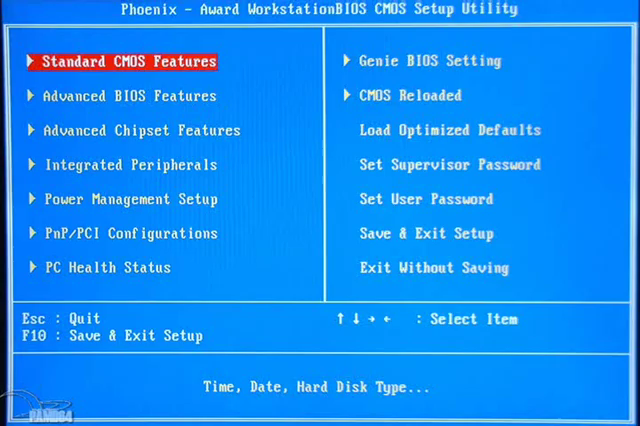
\includegraphics[scale=0.6]{img/00.png}
				\caption{La pantalla principal del CMOS Setup.}
			\end{figure}

		\subsubsection{Standard CMOS Setup}{\label{sub:Standard cmos setup}}
	
			``Standard CMOS Setup'' proviene del Ingles y significa literalmente:
			Configuración estándar de CMOS
			\begin{figure}[H]
				\centering
					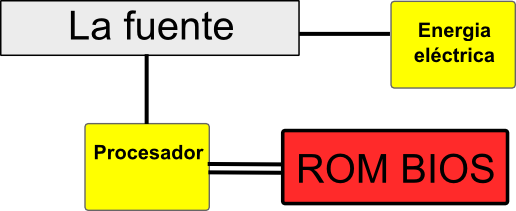
\includegraphics[scale=0.5]{img/01.png}
				\caption{La pantalla del ``Standard CMOS Setup''.}
			\end{figure}
			
			\begin{description}
				\item[Date] Asigna al sistema una fecha. El rango del mes es 1-12, del día 1-31 y del año 1994-2079.
				\item[Time] El formato es de 24 H, ejemplo la 1 de la tarde seria: 13: 00: 00.
				\item[Hard disk] {\emph Disco duro} - La BIOS soporta un
					DUAL-CHANNEL PIO y PCI BUS MASTER IDE. Cada puerto soporta
					una unidad maestra y otra esclava.

					{\large Explicación de las especificaciones de disco duro:}
                
					\begin{description}
						\item[Type] La BIOS contiene una tabla de tipos
							predefinidos. Si no coincide ninguna serie de
							valores, escoger USER.
						\item[Size] Capacidad aproximada del disco. Este tamaño
							suele ser ligeramente mayor que la capacidad una
							vez formateado el disco.
						\item[Cyls] Número de cilindros.
						\item[Head] Número de cabezas.
						\item[Precomp] Cilindro de precompensación de
							escritura. Este parámetro no tiene valor en los
							discos modernos.
					    \item[Landz] Zona de parada. Sólo para discos antiguos sin auto-aparcamiento.
					    \item[Sector] Número de sectores.
						\item[Mode] Auto, Normal, Large, o LBA\footnote{LBA
							(siglas de logical block addressing, dirección
							lógica de bloques) es un método muy común usado
							para especificar la localización de los bloques de
							datos en los sistemas de almacenamiento,
							principalmente secundario, del ordenador. El
							término LBA puede referirse también a la dirección
							del bloque al que enlaza.  Los bloques lógicos en
							los ordenadores modernos son normalmente de 512 o
							1024 bytes cada uno.}

						\begin{itemize}
							\item Auto: La BIOS detecta automáticamente el modo
								óptimo.  \item Normal: El número máximo de
								cilindros, cabezas y sectores soportado es
								1024, 16, y 63.
							\item Large: Discos que no soportan modo LBA y
								tienen más de 1024 cilindros. Solo unos pocos
								discos duros soportan este modo.
							\item LBA (Logical Block Addressrng): Durante los
								accesos a disco, la controladora IDE transforma
								la dirección de datos marcada por el número de
								sector, cabeza y cilindro en la dirección de
								bloque física, mejorando sensiblemente la tasa
								de transferencia de datos. Sólo para discos de
								más de 1024 cilindros.
						\end{itemize}
					\item[Floppy drives A \& B] Selecciona el tamaño de tu
						unidad de diskettes. Las opciones son: 360 KB (5.25”),
						720 KB (3.5”), 1.2 MB (5.25”), 1.44 MB (3.5”), 2.88 MB
						(3.5”).
					\item[Vídeo] Selecciona el tipo de adaptador de
						vídeo de tu PC. Estas son las posibilidades: EGA/VGA,
						MONO, CGA A 40 y CGA A 80.
					\item[Halt on] Durante el chequeo al encender el PC (POST),
						la BIOS se detiene si detecta algún error de hardware.
						Se puede indicar a la BIOS que ignore ciertos errores y
						continúe el proceso de arranque.

					\end{description}
				\end{description}

		\subsubsection{BIOS Features Setup}{\label{sub:bios features setup}}
			\begin{figure}[H]
				\centering
					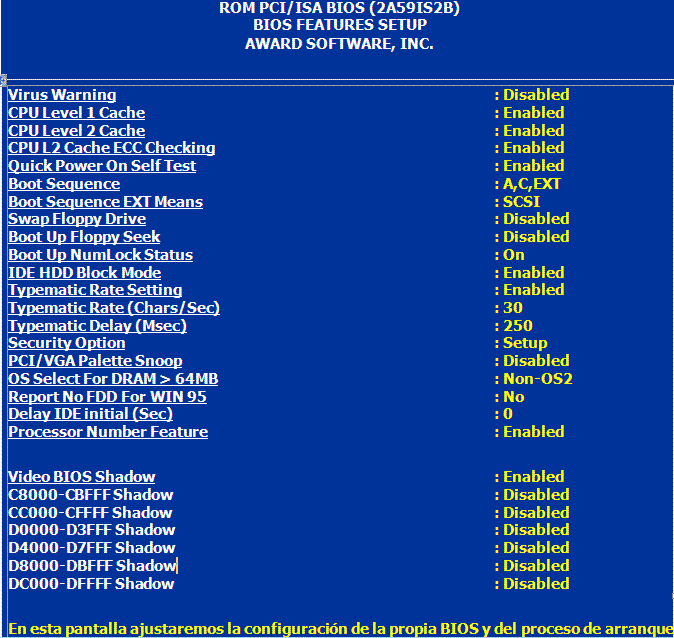
\includegraphics[scale=0.5]{img/02.png}
				\caption{``BIOS Features Setup''}
			\end{figure}
			
			\begin{description}
				\item[Virus Warning] Para impedir que algún soft borre el
					sector de arranque. Recomiendo DISABLE (Usar antivirus).
				\item[CPU Internal caché/External caché] Los datos almacenados
					en memoria caché se transfieren más rápidos, por ello ambas
					opciones deben estar ENABLED.
				\item[CPU L2 Caché ECC Checking] Si este parámetro está
					ENABLED, el procesador dota de un nivel extra de seguridad
					a los datos.
				\item[Quick Power On Self Test] ENABLED, reduce el tiempo
					necesario para realizar el chequeo de arranque (POST). Esto
					omite ciertos pasos. Es preferible que esté DISABLED.
				\item[Boot Sequence] Esta opción ordena, de entre varias
					opciones, la secuencia de arranque. Estas son las opciones
					disponibles: A, C, D, E, F, CD-ROM, SCSI y LS120 / ZIP.
				\item[Swap Floppy Drive] Asigna a la unidad A la letra B y
					viceversa, para ello deben estar las dos disqueteras
					ENABLED.
				\item[Boot Up Floppy Seek] Determina, si está ENABLED, si un
					diskette tiene 40 u 80 pistas. Sólo los diskettes de 360 KB
					tienen 40 pistas, por ello recomiendo DISABLED.
				\item[Boot Up Numlock Status] Activa o Desactiva la tecla Bloq
					Núm.
				\item[Boot Up System Speed] High, arranca a la velocidad por
					defecto del procesador, Low lo hace a la velocidad del BUS
					AT.
				\item[Gate A20 Option] La puerta A20 se refiere a como el
					sistema se comunica con la memoria por encima de 1MB
					(memoria extendida). Cuando se selecciona FAST, el chipset
					del sistema controla la puerta A20. Cuando se selecciona
					NORMAL, lo hace la controladora de teclado. Seleccionando
					FAST, la velocidad del sistema mejora, especialmente en
					OS/2 y Windows.
				\item[Typematic Rate Setting] DISABLED aplicaría los valores
					detallados más abajo y las teclas repetirían con frecuencia
					marcada por la controladora de teclado del sistema. Con
					ENABLED, se puede seleccionar el retraso y la frecuencia de
					repetición.
				\item[Typematic Rate (Chars/Sec)] Con ENABLED se selecciona el
					número de veces por segundo que se repite el caracter de
					una tecla pulsada.
				\item[Typematic Delay (Misc)] Con la opción Typematic Rate
					Setting ENABLED, podemos seleccionar el retraso en
					milisegundos hasta que una tecla pulsada empieza a repetir.
				\item[Security Option] Si se ha establecido una clave, debemos
					seleccionar si se pedirá cada vez que arranque el sistema
					(SYSTEM) o cuando se accede a la configuración (SETUP).
				\item[PCI/VGA Palette Snoop] Sólo se ha de dejar ENABLED si una
					tarjeta ISA instalada en el sistema lo requiriera, para
					sincronizar la tarjeta descompresora MPEG con la tarjeta
					gráfica o si se usa un convertidor VGA/TV.
				\item[OS Select from DRAM>64 MB] Se selecciona si el sistema
					operativo es OS/2 y el equipo tiene más de 64 Mbytes de
					memoria RAM.
				\item[Report No FDD For Win 95] Al seleccionar YES se libera la
					IRQ6 cuando el equipo no tiene disquetera (o no se quiere
					utilizar). Además, debemos deshabilitar el parámetro
					Onboard FDC Controller que podemos encontrar en el submenú
					INTEGRATED PHERIPHERALS de la BIOS.
				\item[Video BIOS Shadow] Pasa la ROM de la tarjeta de vídeo a
					memoria RAM; por lo tanto más rápida.
				\item[C8000 – CBFF/DC – DFFFF Shadow] Más especializado y
					concreto que Video BIOS Shadow, es preferible que esté
					DISABLED.
			\end{description}

		\subsubsection{Chipset Features Setup}{\label{sub:chipset features setup}}
			\begin{figure}[H]
				\centering
					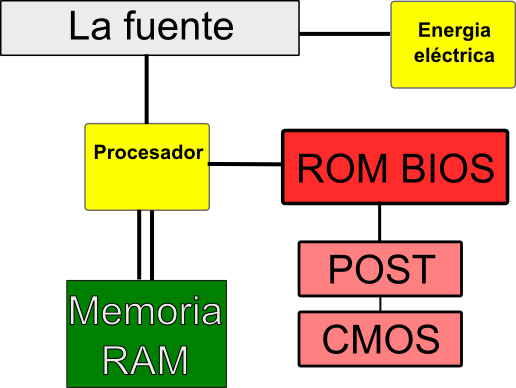
\includegraphics[scale=0.5]{img/03.png}
				\caption{``Chipset Features Setup''.}
			\end{figure}
			
			\begin{description}
				\item[Auto Configuration] Selecciona los valores óptimos
					predeterminados de la velocidad de memoria RAM para los
					parámetros del chipset (FX, HX, VX, TX) de la placa base.
					En caso de estar DISABLED, se vuelve a los valores
					almacenados cuando se instaló la placa base. Si se escoge
					ENABLED, ciertos valores de la sección no pueden
					modificarse. Para modificar estos valores y así obtener el
					máximo de prestaciones del equipo, se debe deshabilitar
					(DISABLED) la autoconfiguración. En algunos equipos no se
					puede deshabilitar.
				\item[EDO DRAM Speed Selection] El valor de este campo debe
					corresponder a la velocidad de la memoria RAM instalada en
					el equipo. NO cambiar los valores por defecto de este campo
					que han sido determinados por el fabricante de la placa
					para la RAM instalada. Este valor es la velocidad de
					acceso, por lo tanto un valor menor implica un equipo más
					rápido.
				\item[EDO CASx MA/RASx Wait State] Sólo para memoria EDO.
					Esto permite al fabricante insertar un estado de espera
					adicional para el refresco de las columnas de memoria. Para
					situar cada bit, el controlador de memoria debe fijar su
					dirección de columna (CAS) y su dirección en fila (RAS).
					Estos valores deben dejarse como están. Si se cambian y
					producen errores de memoria; debemos volver a los valores
					originales.
				\item[SDRAM RAS-to-CAS Delay] Este apartado permite insertar un
					ciclo de retraso entre las señales STROBE de CAS y RAS
					cuando se escribe, lee o refresca la memoria RAM.
				\item[SDRAM RAS Precharge Time] Si se establece tiempo
					insuficiente para que RAS acumule su carga antes del
					refresco de memoria RAM, el refresco puede ser incompleto y
					se pueden perder datos.
				\item[SDRAM CAS Latency Time] Cuando se instala memoria RAM
					síncrona (SDRAM), el número de ciclos de reloj de latencia
					CAS depende de la velocidad de memoria RAM. En general un
					valor menor aumenta las prestaciones y un valor mayor
					incrementa la estabilidad (Esto es aplicable para los tres
					últimos apartados).
				\item[SDRAM RAS Precharge Control] Si está ENABLED los ciclos
					de reloj refrescan todos los bancos de memoria. Estos
					cuatro últimos apartados sólo tienen valor cuando el
					sistema tiene instalada memoria SDRAM.
				\item[DRAM Data Integrity Mode] Selecciona el modo de
					corrección (paridad PARITY, o código de corrección de
					errores ECC) de acuerdo con el tipo de memoria RAM
					instalada.
				\item[System BIOS Cacheable] ENABLED permite copiar a la
					memoria caché la ROM BIOS del sistema en la dirección
					F0000h-FFFFFh, aumentando así las prestaciones. Sin
					embargo, si un programa escribe en este área se puede
					producir un error.
				\item[Video BIOS Cacheable] Permite copiar (ENABLED) a la
					memoria caché la ROM BIOS de la tarjeta gráfica aumentando
					las prestaciones.
				\item[Video RAM Cacheable] Aloja la caché de la tarjeta gráfica
					a la dirección A000 y B000 dentro de la memoria RAM; siendo
					así más rápida.
				\item[8/16 Bit I/O Recovery Time] Estos dos campos permiten
					añadir tiempo de recuperación (en ciclos de reloj del bus)
					para las órdenes de entrada y salida de los dispositivos
					ISA de 8 y 16 bits. En general, cuanto menor es el número
					mejores son las prestaciones, aunque deben hacerse pruebas
					con los valores seleccionados.
				\item[Memory Hole At 15M-16M] Se puede reservar este área de la
					memoria del sistema para la memoria ROM de las tarjetas
					ISA. Si se reserva, no se puede utilizar como caché. Ver el
					manual de los dispositivos por si lo necesitan.
				\item[Passive Relase] Esta función se utiliza para que puedan
					realizarse los accesos del procesador al bus ISA. Es
					recomendable habilitar o desahibilitar si se tienen
					problemas de compatibilidad con una tarjeta ISA.
				\item[Delayed Transaction] El chipset tiene un buffer de
					escritura de 32 bits para soportar ciclos retardados de
					transacciones. Selecciona ENABLED para que esté de acuerdo
					con la versión 2.1 del bus PCI. ENABLED mejora las
					prestaciones del equipo.
				\item[AGP Aperture SIZE (MB)] Selecciona el tamaño de apertura
					del Puerto de Gráficos Acelerados.  La apertura es una
					parte del rango de la dirección de memoria PCI dedicada
					para el espacio de dirección de la memoria gráfica.  El
					valor más habitual es 64MB, se estima que la cantidad
					idónea se obtiene igualando o dividiendo entre dos la
					memoria RAM instalada en el equipo.
				\item[CPU Host Clock] Por defecto viene en AUTO, pero podemos
					escoger las combinaciones: AUTO, 100, 103, 112 y 133 Mhz.
				    Estas son las frecuencias adecuadas que debemos combinar: \\ 

					\begin{tabular}{ l | c | c | c | r }
						\hline
	Frecuencia Ext. &      AGP         &    PCI    &    ISA    & DIMM \\ 
						\hline
	100 Mhz         &      66 Mhz      &  33 Mhz   &  8.33 Mhz & 100 Mhz \\ 
	103 Mhz         &     68.6 Mhz     & 34.3 Mhz  &  8.33 Mhz & 103 Mhz \\
	112 Mhz         &     74.6 Mhz     & 37.3 Mhz  &  8.33 Mhz & 112 Mhz \\ 
	133 Mhz         &    88.67 Mhz     & 44.33 Mhz &  8.33 Mhz & 133 Mhz \\ 
						\hline
					\end{tabular}
					
			\end{description}
			\newpage
			
		\subsubsection{Power Management Setup}{\label{sub:power management setup}}
			\begin{figure}[H]
				\centering
					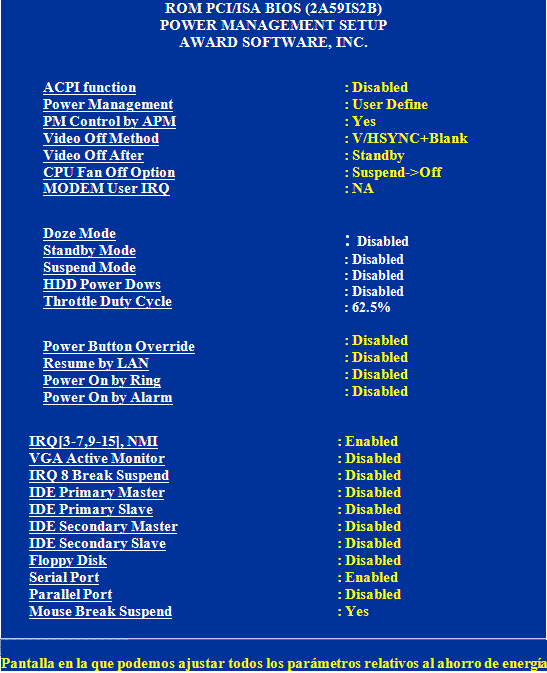
\includegraphics[scale=0.5]{img/04.png}
				\caption{``Power Management Setup''.}
			\end{figure}
				
			\begin{description}
				\item[Power Managament] Permite escoger el tipo o grado de
					ahorro de energía entre los modos Doze, Standby y Suspend.
					Esta tabla describe cada uno de los modos:

					\begin{tabular}{| l | r |}
						\hline
		 Max Saving  & Ahorro máximo. Sólo para procesadores SL (portátiles). \\ 
		 User Define & Establecer individualmente cada modo. \\ 
		 Min Saving  & Ahorro mínimo. \\ 
						\hline
					\end{tabular}
				\item[PM Control by APM] Seleccionando YES, el sistema avanzado
					de energía (APM), mejora el ahorro.
				\item[Video Off Method] Sistema para indicarle al monitor que
					debe entrar en un modo de ahorro de energía. Recomiendo:
					que sea consultado el manual del periférico para un ajuste
					optimo.  Estas son las opciones disponibles: DPMS OFF, DPMS
					reduce ON, Blank Screen, V/H SYNC+Blank, DPMS Standby, DPMS
					Suspend.
				\item[Video Off After] Esta opción permite que el monitor se
					adapte (se limpie) después de que el sistema haya entrado
					en Doze, Standby o Suspend mode. Se puede deshabilitar esta
					opción con el parámetro N/A. Por defecto el valor es
					Standby.
				\item[MODEM use IRQ / Wake up on LAN] Opciones que especifican
					la interrupción asignada al módem y si al detectar una
					llamada debe encenderse el sistema.
				\item[Doze Mode] Después del tiempo de inactividad
					seleccionado, el reloj del procesador va más lento aunque
					el resto de los componentes todavía operan a toda
					velocidad.
				\item[Standby Mode] Después del periodo de tiempo seleccionado,
					el disco duro y la tarjeta gráfica se apagan mientras que
					los otros dispositivos siguen funcionando.
				\item[Suspend Mode] Después del periodo de inactividad
					seleccionado, todos los dispositivos excepto el procesador
					se apagan.
				\item[HDD Power Down] Después del tiempo seleccionado de
					inactividad, el disco duro se apaga pero los otros
					dispositivos no.
				\item[Throttle Duty Cycle] Cuando el sistema entre en modo
					Doze, el reloj del procesador corre sólo parte del tiempo.
					Aquí se puede seleccionar el porcentaje de ese equipo.
				\item[PCI/VGA Act-Monitor] Habilita o deshabilita la detección
					de inactividad del monitor.
				\item[Soft-Off by PWR-BTTN] Pone al equipo en un modo de muy
					bajo consumo, Instand-off hace que vuelva inmediatamente a
					estar disponible al tocar el botón ON/OFF o recibir una
					llamada por el módem. Con Delay 4 Sec., el sistema espera 4
					segundos antes de hacer todo lo anterior.
				\item[CPUFAN off In Suspend] El ventilador del procesador se
					apagará cuando este esté inactivo.  Resume by Ring: Una
					llamada al módem anula el modo de ahorro de energía.
				\item[Resume by Alarm / Date (of Month) Alarm, Time (hh:mm:ss)
					Alarm] Con el primer parámetro habilitamos o deshabilitamos
					al segundo, que permite establecer la fecha y hora para que
					el equipo despierte del modo suspendido.
				\item[IRQ 8 Break Suspend] Se puede habilitar o deshabilitar la
					monitorización de la IRQ8 (Real Time Clock, Reloj en tiempo
					real) para que no anule el modo Suspend de ahorro de
					energía.
				\item[Reload Global Timer Events] Cuando está ENABLED cualquier
					operación de los dispositivos listados reinicia el
					temporizador para el modo Standby.
			\end{description}
			\newpage
		\subsubsection{PNP/PCI Configuration}{\label{sub:pnp/pci configuration}}
			\begin{figure}[H]
				\centering
					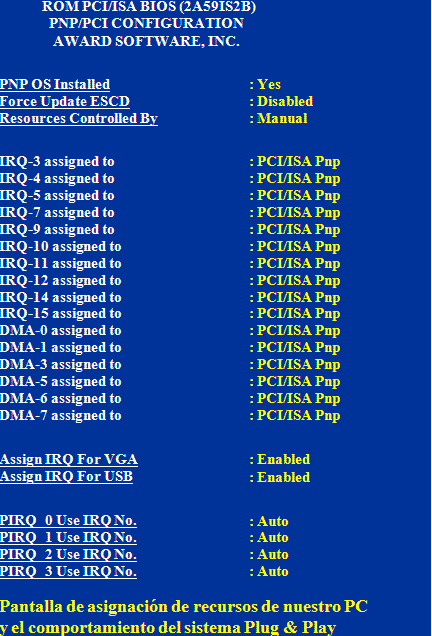
\includegraphics[scale=0.5]{img/05.png}
				\caption{``Configuracion de PNP/PCI''.}
			\end{figure}
			\begin{description}
				\item[PNP OS Installed] Activar siempre que se haya instalado un
					sistema operativo PnP. 
				\item[Resources Controlled By] La BIOS de tipo Plug and Play
					configura automáticamente los dispositivos que cumplen
					dicho estándar. Si se selecciona AUTO, desaparecen los
					campos IRQ y DMA, porque la BIOS los asigna
					automáticamente.
				\item[Reset Configuration Data] Normalmente este valor está
					DISABLED. Se selecciona ENABLED para reiniciar los datos de
					configuración al salir de la BIOS, después de haber
					instalado un dispositivo o haber cambiado valores debido a
					un fallo en el encendido del equipo.
				\item[IRQ-xx assigned to / DMA-x assigned to] Estos parámetros
					reservan IRQ (petición de interrupción) o canales DMA
					(acceso directo a memoria) a ciertos dispositivos. Si
					tenemos una tarjeta ISA y esta no es PnP, requiere una
					interrupción IRQ o un canal DMA que soporten esa función,
					para ello debemos asignar a los susodichos IRQ o DMA la
					opción “Legacy ISA”.
				\item[Used MEM base addr] Este parámetro, en conjunción con
					“Used MEM Length” asignan la dirección base para el área de
					memoria usada por cualquier periférico que requiera memoria
					alta (de 640 KB a 1 MB).
				\item[Assign IRQ For USB] Por defecto viene ENABLED. Se puede
					Deshabilitar si necesitamos alguna IRQ extra y carecemos de
					dispositivos USB que las ocupen.
			\end{description}

		\newpage

	\subsection{Restaurar la configuración del CMOS Setup}{\label{sec:cmossetup/resetear-el-cmos-setup}}

		Hay varias formas de restaurar la configuración del CMOS Setup o bien del chip CMOS. \\
		Generalmente no se lo hace, pero en caso de olvidar la contraseña de acceso

	\subsubsection{Batería CMOS}{\label{sec:bateria cmos}}

		Sacar la pila del CMOS que se encuentra sujetada en un slot para la pila en
		la placa base por unos segundos, despues reemplazarla otravez.

	\subsubsection{El RESET CMOS}\label{sec:el reset cmos}

	\begin{figure}[H]
		\centering
			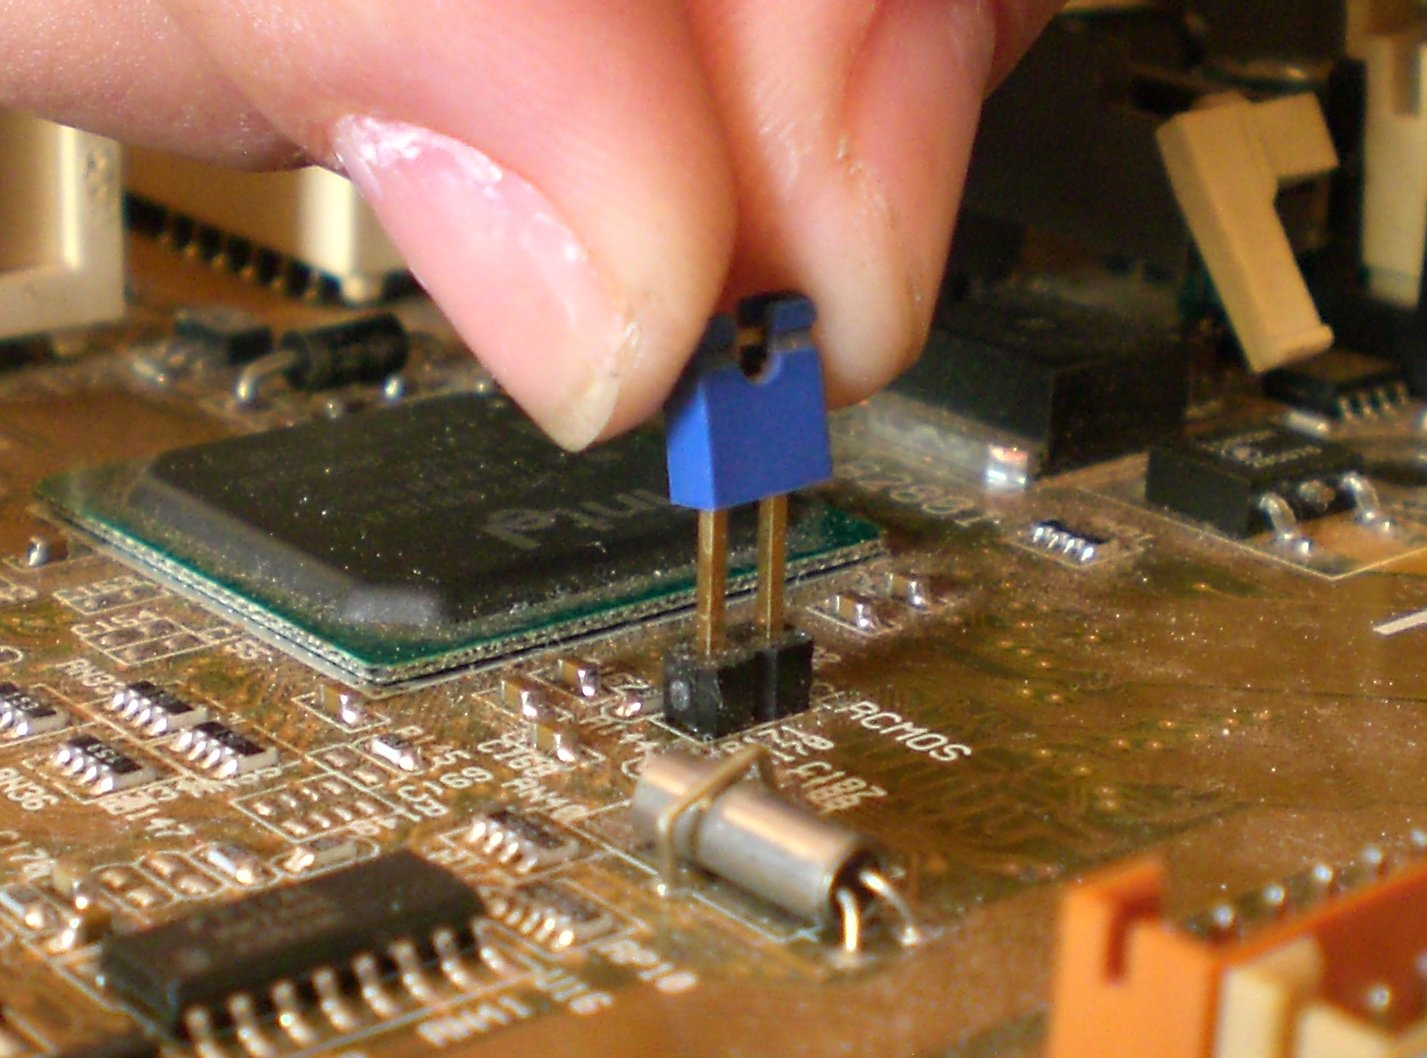
\includegraphics[scale=0.2]{img/RESET_CMOS.JPG}
		\caption{El ``RESET CMOS''}
	\end{figure}
	Algunas placas base ofrecen un jumper CMOS-reset o un botón de reinicio.

	\subsubsection{Metodo programativo}\label{sec:metodo programativo}

	En otros casos, el chip EEPROM ha de desoldar los datos en forma manual,
	por manos de un programador. 
	A veces es suficiente motivo para el CLK o línea de DTA de la I2C bus de la
	EEPROM en el momento adecuado durante el arranque, esto requiere una cierta
	precisión en las piezas de soldadura SMD. 
	Si la máquina le permite arrancar, pero no quiere que le permiten a la
	configuración de la BIOS, una posible recuperación es dañar la suma de
	comprobación CMOS, haciendo puerto directo escribe usando debug.exe,
	corrompiendo a algunos bytes de la suma de control de área protegida de la
	RAM CMOS, en el siguiente arranque, el equipo normalmente restablece su
	configuración de fábrica. Por ejemplo:

	\begin{verbatim}
	c:\debug
	-o 70 10
	-o 71 aa
	-q
	\end{verbatim}

	Que permitirá escribir en CMOS (Offset 10h) con el valor 0AAhA.

	\newpage

\appendix

